\documentclass[12pt]{article}
\usepackage[utf8]{inputenc}
\usepackage[russian]{babel}
\usepackage{graphicx}
\usepackage{placeins}
\graphicspath{{proteus/}}
\title{Курс молодого бойца}
\author{Ушаков А. Е., Храмцов И. А., Кузнецов В. А.}
\date{\today}
\begin{document}



\maketitle


\newpage
\tableofcontents
\newpage
\section{Необходимый список программ}
\begin{itemize}
\item Atmel Studio 6
\newline Это весьма популярная среда программирования для контроллеров Atmel, предоставляется бесплатно.
\newline $http://www.atmel.com/tools/atmelstudio.aspx$
\item ChipProg Usb
\newline Среди оборудования ЛЭМФ есть программатор ChipProg40, способный программировать в параллельном режиме почти любой микроконтроллер.
Из-за его устройства наиболее удобно программировать микроконтролеры в DIP корпусе.
Сама программа устанавливается и запускается только при наличии подключенного к компьтеру программатора.
Иструкция к программе имеется на сайте разработчика.
\newline $http://www.phyton.ru/download/$
\item Sprint-Layout
\newline Простой, но в тоже время очень эффективный программный пакет для проектировки и ручной разводки печатных плат малой и средней сложности.
\newline $http://cxem.net/software/sprint\_layout.php$
\item Proteus (для моделирования всего и вся) Ссылку находить на торрентах:)
\end{itemize}
\section{Справочный материал}
\begin{itemize}
\item Atmega8a DataSheet
\newline Здесь можно найти всю информацию по распиновке контроллера, написания кода на C и ассемблере и прошивке.
\newline $http://www.atmel.com/images/atmel-8159-8-bit-avr-microcontroller-atmega8a\_datasheet.pdf$
\item Г. И. Донов "Применение микроконтроллеров"
\newline Эту книгу можно взять в библиотеке. Будет полезна тем, кто не хочет читать новый материал из даташита выше сразу на английском.
\item Информация по изготовлению печатных плат методом ЛУТ 
\newline $http://easyelectronics.ru/sozdanie-pechatnoj-platy-metodom-lazernogo-utyuga.html$
\item Руководство по разведению печатных плат с помощью программы SprintLayout 5.
\newline $http://easyelectronics.ru/sprint-layout-5-podrobnoe-rukovodstvo.html$
\item По оппонентной теории Геринга можно прочитать в дипломах А. Баранова и Е. Евдокимова. Они есть у А. И. Миланича.
\end{itemize}

\section{Оборудование ЛЭМФ}
В лабаратории есть некоторое количество печатных и макетных плат, которые мы здесь перечисляем.
\begin{itemize}
\item Макетная плата
\newline Такая же как на РТ лабах.
\item Несколько микроконтролеров Atmega8 в DIP корпусах.
\item Несколько rgb светодиодов.
\item Программатор ChipProg40
\item ISP переходник для программатора. Внимание, может пропадать контакт.
\item Изготовленные методом фрезерования 2 сторониие платы для монтажа схемы со светодиодом и ISP разъёмом.
\end{itemize}

\section{Использование программ}
\subsection{Proteus}
После запуска Proteus(isis.exe) должно открыться окно как на рис.~\ref{p1} 
\begin{figure}[H]
\center{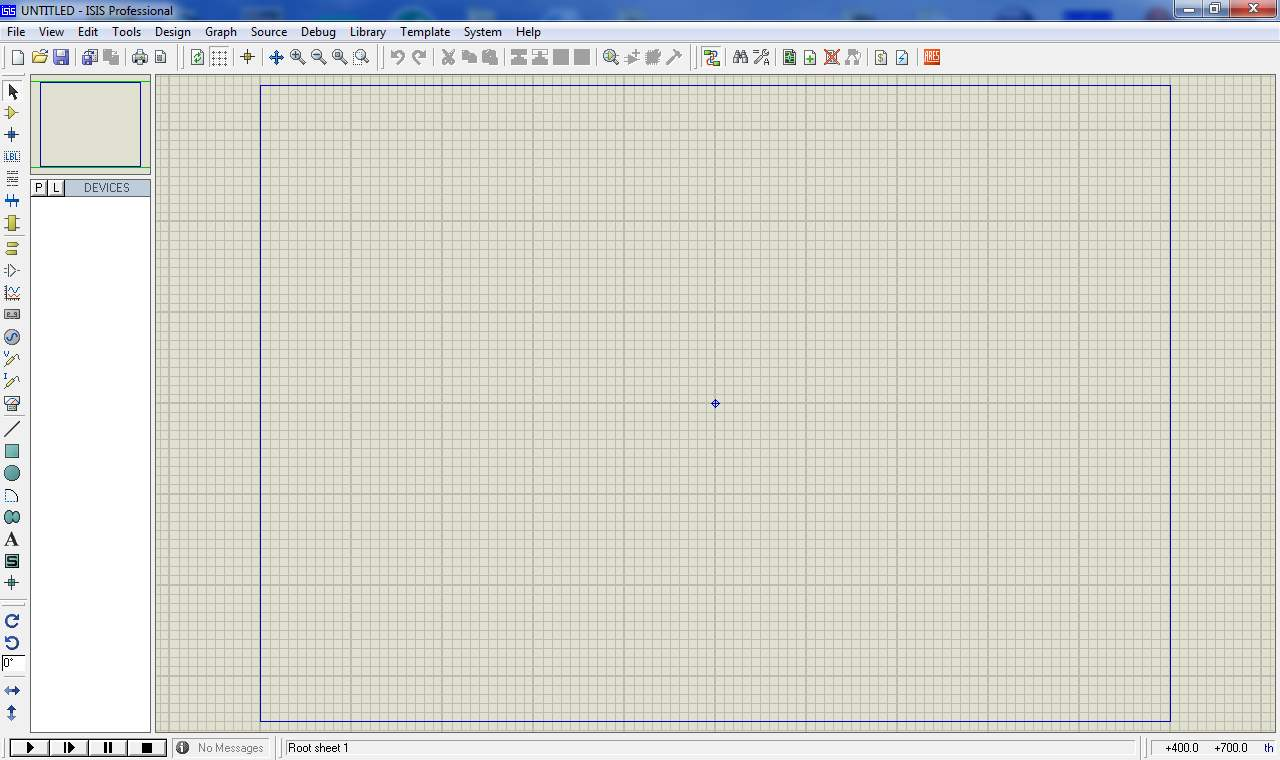
\includegraphics[width=0.8\linewidth]{1.jpg}}
\caption{Начальное окно Proteus}
\label{p1}
\end{figure}
Чтобы выбрать микроконтроллер(или какой либо другой элемент) запустите окно Pick devices. рис.~\ref{p2} 
\begin{figure}[H]
\center{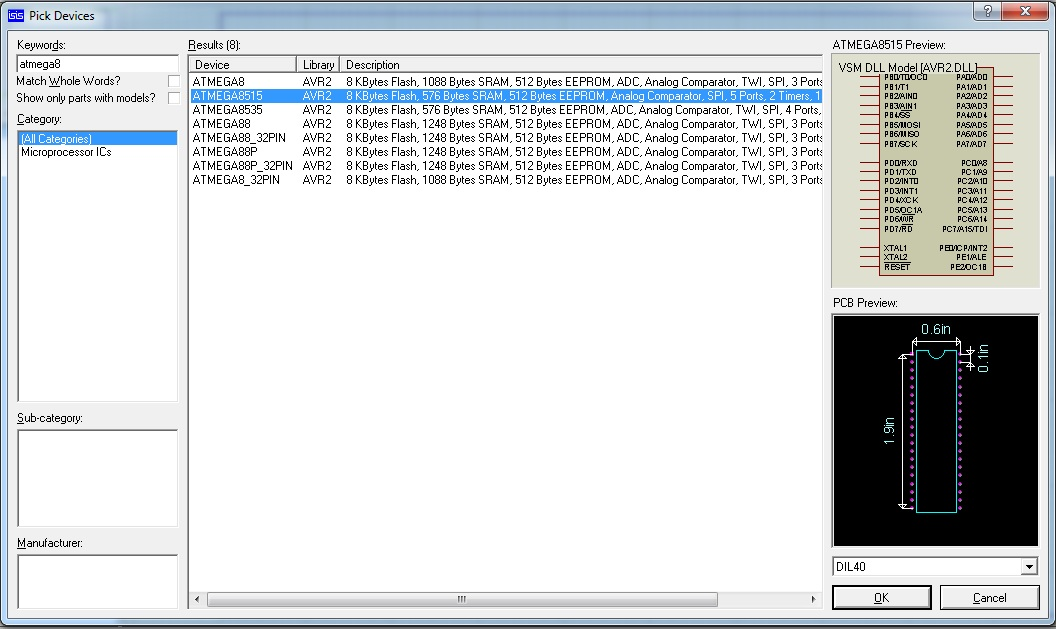
\includegraphics[width=0.8\linewidth]{2.jpg}}
\caption{Pick devices}
\label{p2}
\end{figure}
Прошить микроконтроллер можно, выбрав соответствующий hex файл, в Edit component рис.~\ref{p3} 
\begin{figure}[H] 
\center{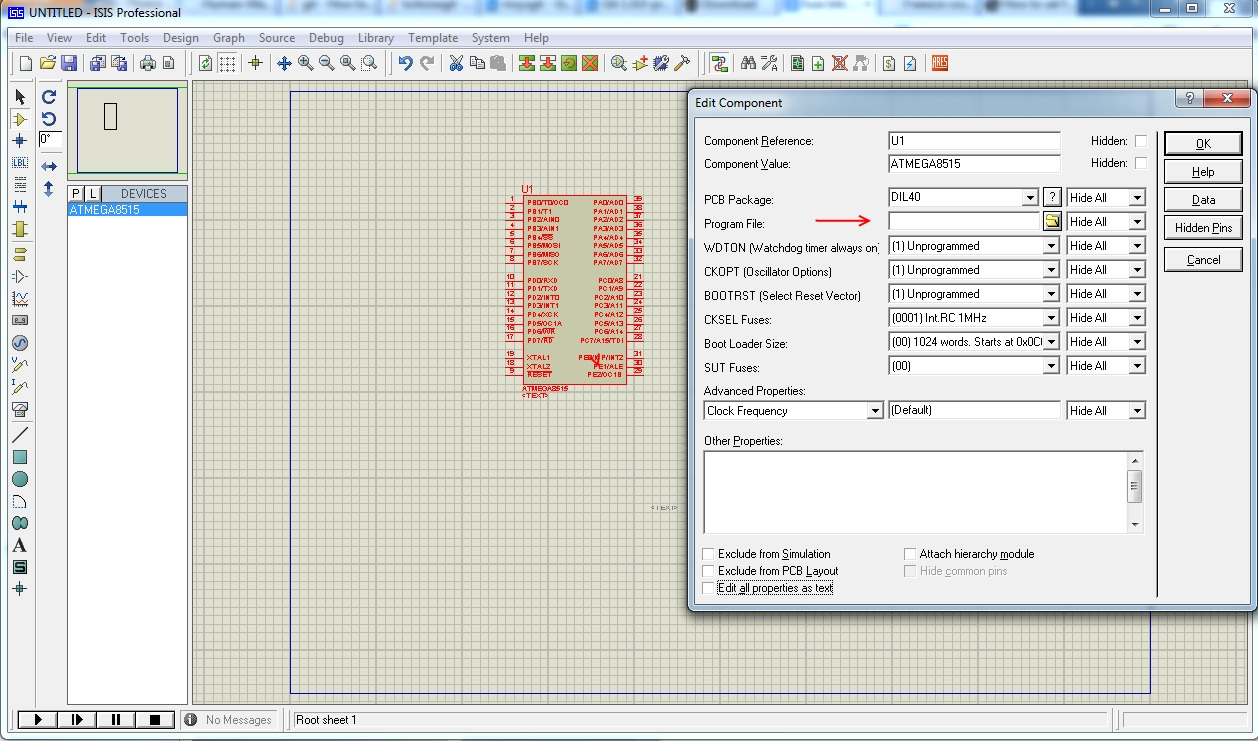
\includegraphics[width=0.8\linewidth]{3.jpg}}
\caption{Pick devices}
\label{p3}
\end{figure}

\newpage
\FloatBarrier
\section{Куски кода}

\subsection{}
\subsection{}
\subsection{Usart и еже с ним}
\subsection{}
\end{document}
